\clearpage
\section{Introduction}
\label{sec:search-introduction}

The minimal supersymmetric Standard Model (MSSM) has been significantly constrained by searches for new physics carried out by the CMS and ATLAS experiments in Run 2. However, the underlying considerations that motivate these searches remain a significant puzzle. The identity of most of the mass of galaxies as inferred by observations of galactic rotation, as well as by analysis of the CMB, remains unknown. The apparent coincidence known as the large hierarchy problem, whereby the series of $\mathcal{O}(\Lambda^2)$ loop contributions to the mass of the SM Higgs boson vanishes, remains without a demonstrated underlying mechanism to explain the vanishing "naturally." The MSSM, as well as supersymmetry at large, endures as a well-motivated candidate extension of the SM to the extent that theoretical phase space with explanatory power for the issues above remains non-excluded by experimental observations. It is therefore a pertinent exercise to identify any such remaining regions, and to design and implement experimental methods to either rule them out or perhaps observe signals indicating their manifestation. 

In the MSSM, the SM is extended to contain two Higgs doublets, with supersymmetric partners of the Higgs bosons called Higgsinos. These Higgsinos mix with the gauginos, winos and binos, to form the charginos and neutralinos mass eigenstates, also referred to as electroweakinos, as described in Section~\ref{sec:MSSM}. The lightest neutralino, \PSGczDo, is assumed to be the lightest SUSY particle (LSP), which is stable due to R-parity conservation. That makes the LSP a good WIMP candidate for DM. In this search, a scenario where the lightest electroweakinos, \PSGczDt, \PSGcpmDo, \PSGczDo, are dominated by the Higgsino component is considered. The DM candidate in this case is also referred to as a nearly pure higgsino LSP with little-to-no mixing from other states. This corresponds to the condition that the Higssino mass parameter $\mu$ is much smaller than the magnitude of the bino and wino mass parameters $M_1$ and $M_2$, \ie, $\abs{\mu}\ll \abs{M_1},\abs{M_2}$. This scenario is motivated by naturalness arguments~\cite{BARBIERI198863,de_Carlos_1993}. A hallmark feature of higgsinos is the particle mass spectrum, comprising a 4-fold nearly mass degenerate group of electroweakinos, namely $\tilde{\chi}_{1,2}^{0}$ and $\tilde{\chi}_{1}^{\pm}$. This mass degeneracy is referred to as a compressed mass spectrum. A careful treatment of radiative corrections is needed to properly account for a large difference between the higgsino mass and the SUSY breaking scale \cite{Nagata_2015}, which is the case for such low-mixing scenarios. These calculations establish a lower limit on the mass difference between the LSP and lightest chargino state $\Delta m^{\pm}=\Delta m(\tilde{\chi}_{1}^{0},\tilde{\chi}_{1}^{\pm})$ of around 250 MeV for $m(\tilde{\chi}_{1}^{0})=100$ GeV, increasing gradually with larger LSP mass. This bound corresponds to the no-mixing limit; any mixing between the higgsino and the wino or bino states gives rise to larger values of $\Delta m^{\pm}$. 

The analysis is optimized with respect to scenario above under the assumption that the mass difference between the two neutral higgsino states $\Delta m^{0} = \Delta m(\tilde{\chi}_{2}^{0}, \tilde{\chi}_{1}^{0})$ is twice the value of that between the charged and lightest states: $\Delta m^{0} = 2\Delta m^{\pm}$. This is consistent with the limit of large tan$\beta$. Two production processes dominate the total cross section, and are shown in Fig. \ref{fig:signal-feynman-diagrams}. This search targets final states containing two soft (small momenta) same-flavor opposite-charge leptons and a large magnitude of missing transverse momentum. Since the decay products can have very low momentum, sometimes a lepton is not successfully identified, and a track is used in its place. Experimental constraints in these compressed scenarios are limited by the small momenta of the visible decay products, as well as by small electroweak production cross-sections. The scenario described here is realized as a simplified model, in which particle masses for particles which are not considered in this model are set to infinity~\cite{Chatrchyan_2013}.

\begin{figure}[h]
\centering
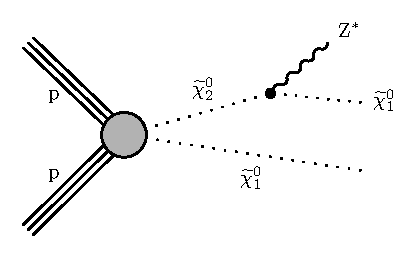
\includegraphics[width=0.48\linewidth]{plots/feynman_diagrams/gitTChiZ.pdf} \,
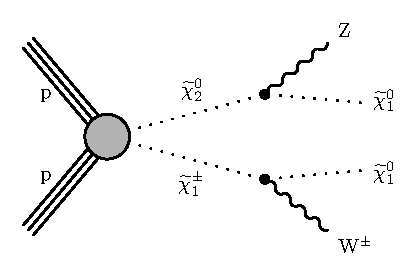
\includegraphics[width=0.48\linewidth]{plots/feynman_diagrams/gitTChiWZ.pdf}  \\
\caption[Signal Models Feynman Diagrams]{Production and decay of electroweakinos in the higgsino simplified model through \tchiz (left) and \tchiwz (right). }
\label{fig:signal-feynman-diagrams}
\end{figure}